\chapter{Introduction}

\section{Financial Contracts}

In the real world, two parties may create a \textit{financial contract} to describe a set of payments to be made between them under certain conditions. These contracts can suffer from numerous issues in real world usage; for one thing, the financial world is plagued with jargon, which can make contracts difficult to interpret, and complicated to compose. This can lead to unneeded verbosity, where certain terms may be repeated multiple times in a single contract. Traditional financial contracts can also be difficult to analyse mathematically in terms of potential cost or value, due to their complexity and potential ambiguity - resulting in the appearance of unnoticed errors in contract definitions.

\section{A Combinator Domain-Specific Language to Represent Contracts}

A hypothetical solution to alleviate some of these issues has been proposed by Simon Peyton Jones, Jean-Marc Eber, and Julian Seward in the paper \textit{Composing Contracts: An Adventure in Financial Engineering}\cite{SPJ}. Their proposed solution employs a combinator domain-specific language, which is a type of functional programming language where specific terms, i.e. \textit{combinators}, can be composed to produce a program. This solution involves using combinators to represent financial contracts. This is possible as these financial contracts can typically be described such that they are composed of smaller contracts - i.e. \textit{sub-contracts}. These combinators can be as simple as \texttt{one}, which requires the counter-party to pay a single unit of a given currency to the owner. They can also describe transformations on inner combinators, such as \texttt{scale}, which multiplies any monetary values in inner combinators by a given value. The contract \texttt{scale(5, one(GBP))} will therefore require the counter-party to pay the owner \pounds 5. \\

The definition of financial contracts using a combinator DSL has numerous upsides. For one thing, even with few combinators a contract writer can define a huge variety of financial contracts, thus reducing the amount of jargon required. If any contracts which cannot be represented by the combinator DSL are found, new combinators can easily be added due to their modular nature. Programmatic definition of financial contracts can also cut down on needless repetition, and there is no room for interpretation. Additionally, the use of combinators facilitates mathematical analysis of financial contracts' values, by the composable nature of these values - where each combinator's value is a function of their inner combinators' values. While there is an implementation of an evaluation process for financial contracts written in the DSL, there is no programmatic implementation of these contracts.

\section{Smart Contracts}

Since the original DSL was first described, cryptocurrencies have proliferated; because of this, it has become popular to represent financial contracts using \textit{smart contracts}. Smart contracts are programs which can be deployed to a blockchain, and then called at any time to execute some specified code. One specific functionality they provide is the ability to obtain and transfer cryptocurrencies, thus facilitating payments between multiple parties under specified conditions in an automated manner\cite{Eth}. Writing smart contract representations of financial contracts allows financial institutions to use blockchains between institutions for payment of funds according to these financial contracts, or simply to keep track of existing financial contracts for auditing purposes thanks to the immutability of blockchains. \\

While existing smart contract languages can provide a strict and unambiguous smart contract representation of a financial contract, i.e. a \textit{financial smart contract}, there are issues with this manner of implementation. One such issue is that many smart contract languages are exceedingly error-prone, meaning that it is very possible to write a financial smart contract with unintended consequences - in fact, it has been estimated that 45\% of smart contracts on the Ethereum blockchain (a platform for hosting smart contracts) contain vulnerabilities\cite{EthSec}. \\

Take the smart contract code in listing \ref{listing:reentrancy}, written in Solidity (a programming language for smart contracts); this code simply transfers funds from the smart contract to the caller, and then decrements a \textit{balance} representing the funds the caller can withdraw. To the untrained eye (and the Solidity compiler), this code snippet contains no errors; in actuality, it contains one of the most severe kinds of vulnerabilities, allowing a reentrancy attack from a malicious user. A reentrancy attack is where funds are transferred before a function's invocation is finished, allowing the function to be called again before the transfer is complete and the balance is decremented (as transfers can trigger function calls)\cite{eth-known-attacks}. This can result in the smart contract being drained of all of its funds. This is an example of a severe vulnerability that can be easy to miss when implementing smart contracts in a smart contract language. \\

\begin{lstlisting}[language=Solidity, caption=A Solidity function which is vulnerable to a reentrancy attack$^1$., captionpos=b, label=listing:reentrancy]
function withdrawOneWei() public {
    msg.sender.call.value(1);
    balances[msg.sender] = balances[msg.sender] - 1;
}
\end{lstlisting}
\stepcounter{footnote}
\footnotetext{Solidity syntax highlighting obtained from the \texttt{solidity-latex-highlighting} package written by Sergei Tikhomirov, used under the MIT license, available at \url{https://github.com/s-tikhomirov/solidity-latex-highlighting}.}

Smart contracts are also difficult to analyse mathematically in terms of definitive costs, as most smart contract languages are relatively complex (in comparison to the combinator DSL mentioned earlier). Complex functionality like iteration and recursion can make the outcome of program execution difficult to evaluate, and also makes errors relatively easy to introduce and difficult to discover. These features are not required for the representation of financial contracts, as demonstrated by their absence from the aforementioned DSL. Overall, the issues mentioned here make smart contract languages a risky choice when creating financial smart contracts, as it can be easy to allow erroneous behaviour to occur, and difficult to find such errors by analysis.

\section{Our Contributions}

In this work, we present several contributions with the aim of improving the ease of implementation and reducing the risk of erroneous behaviour for financial smart contracts: \\

\begin{enumerate}
    \item \textbf{SmartFin}: A combinator DSL for representing financial contracts, derived from the \textit{original DSL} created by Peyton Jones et al.\cite{SPJ}, with slight modifications to enable a smart contract implementation. The design of SmartFin is detailed in chapter \ref{combinator-DSL}.
    \item \textbf{SmartFin Smart Contract Implementation}: An Ethereum-compatible smart contract that can represent any given SmartFin financial contract as a financial smart contract. The implementation of this smart contract is detailed in chapters \ref{smart-contract-impl} and \ref{combinators-main}.
    \item \textbf{Web Client}: A web client for managing SmartFin smart contracts. The implementation of the web client is detailed in chapter \ref{web-client}. The web client implements the following functionality:
    \begin{itemize}
        \item Composition of SmartFin financial contracts, with syntax verification and detailed error reporting with stack traces.
        \item Evaluation of SmartFin financial contracts in a step-by-step manner, to calculate the value that a contract is worth given all required external input (provided by the user) at each required step. The times that all evaluated payments would occur can also be displayed.
        \item Deployment of SmartFin financial smart contracts to any compatible blockchain.
        \item Monitoring of any deployed SmartFin financial smart contracts state, and displaying this state to a user.
        \item Interaction with deployed SmartFin financial smart contracts, allowing users to provide any input that the financial contract requires. \\
    \end{itemize}
\end{enumerate}

With all of these tools together, a user can define a financial contract in the SmartFin DSL using the web client; this SmartFin financial contract can be evaluated in the web client in a step-by-step manner, or can be passed to the implemented smart contract and deployed to a connected compatible blockchain. The deployed financial smart contract can be monitored and interacted with through the web client, and as such all of the required functionality to use SmartFin financial smart contracts is available in the web client. The implemented smart contract can take any given SmartFin contract definition in its constructor and modify its state so that its behaviour matches the given financial contract's behaviour, by implementing logic for all combinators' semantics. A dependency graph of the contributions implemented is depicted in figure \ref{fig:contributions-block}. \\

\begin{figure}[h]
    \centering
    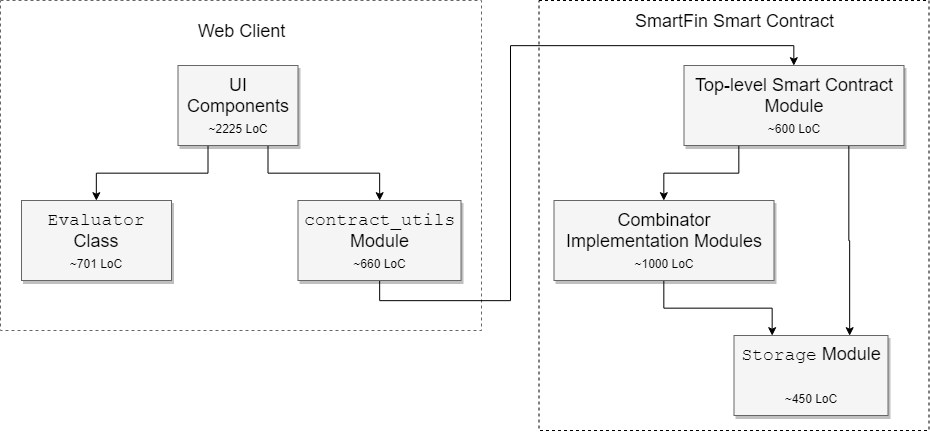
\includegraphics[width=\textwidth]{contributions-block.png}
    \caption{A dependency graph of the modules implemented for this project, with their approximate \textit{Lines of Code} (not including tests).}
    \label{fig:contributions-block}
\end{figure}


\section{Challenges}

\subsubsection{SmartFin Smart Contract Implementation}

Implementing the SmartFin combinator DSL in a smart contract is no small feat; while the number of combinators is relatively limited, representing \textit{any} set of combinators requires a robust generic design when it comes to the implementation of the combinators' semantics and state. Furthermore, this design needed be applicable to \textit{all} combinators, and some are quite unintuitive to represent programmatically. The representation of SmartFin combinators is described in chapter \ref{combinators-main}.

\subsubsection{Ethereum Limitations}

Due to limitations of the Ethereum platform, it is not possible to create a one-to-one representation of a SmartFin contract in smart contract form. Designing solutions to the issues caused by the nature of the Ethereum platform required compromises to be made, and minimising the resulting compromises required designing multiple alternative solutions and evaluating them objectively. Solutions to issues stemming from the Ethereum platform are discussed in chapter \ref{smart-contract-impl}.


\subsubsection{SmartFin Contract Evaluation}

Evaluating SmartFin financial contracts is not a simple problem, even when approaching it in a step-by-step manner, for a couple of reasons. One issue is that SmartFin contracts deal heavily with time, making time an important factor in the evaluation of SmartFin contracts. Keeping track of distinct periods of time based on the SmartFin contract and user interaction was required for step-by-step analysis, requiring a system of describing these time periods to be designed and implemented. Furthermore, keeping track of the current state while requiring the user to enter data can be quite complex, and the ability for the user to revert to any earlier state of step-by-step evaluation can make this even worse. Additionally, the evaluation process requires backtracking for certain combinators, thus resulting in even more complicated behaviour. The implementation of step-by-step evaluation is described in section \ref{client-evaluate}.